\chapter{Arcade Machine Setup}
\label{cha:arcade_machine_setup}

This chapter explains how to assemble the arcade machine hardware and run the system on the Raspberry Pi.

\section{Hardware Assembly}
\label{sec:hardware_assembly}

The hardware assembly stage involves connecting all physical components of the arcade machine. This includes mounting the joysticks and buttons, wiring them to the USB encoder, and linking the encoder and other peripherals to the Raspberry Pi.

\subsection{Installing Joysticks and Buttons}
\label{subsec:installing_joysticks_buttons}
Ensure that the buttons are arranged in a comfortable layout for gameplay. While the layout can be adjusted to personal preference, this project follows the configuration shown below.
\\
\begin{figure}[htb]
  \centering
  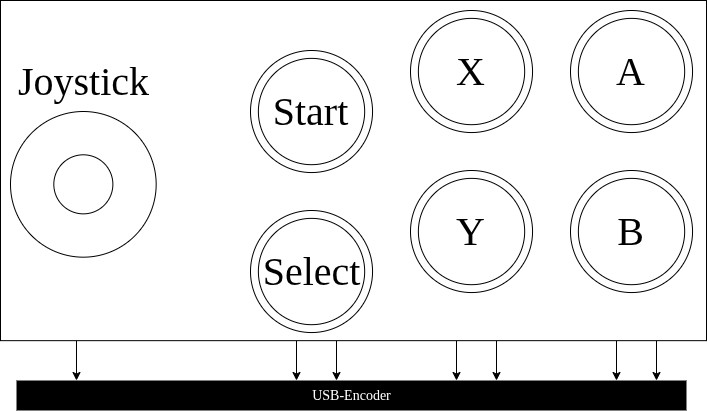
\includegraphics[scale=0.5]{F_Figures/button_layout.png}
  \caption{Joystick and button layout.}
  \label{fig:button_layout}
\end{figure}

\subsection{Connecting USB Encoder}
\label{subsec:connecting_usb_encoder}
Attach the arcade buttons and joystick wires to the USB encoder in accordance with the Figure 3.2. The encoder converts physical inputs into signals recognized by the Raspberry Pi over USB.
Note that the joystick uses 5-pin, arcade buttons use 3-pin cable for connection.
\\
\begin{figure}[htb]
  \centering
  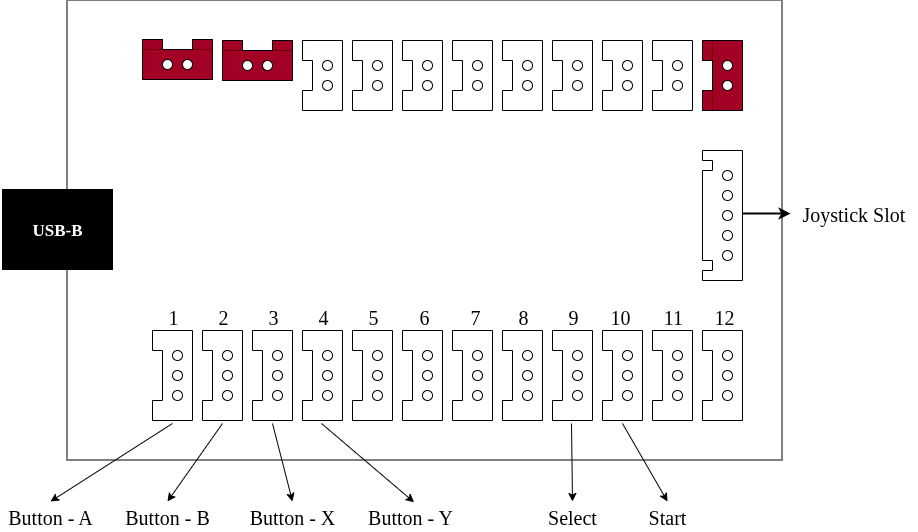
\includegraphics[scale=0.36]{F_Figures/usb_encoder_layout.png}
  \caption{USB-encoder wiring schema.}
  \label{fig:usb_encoder_layout}
\end{figure}

\subsection{Connecting Hardware to Raspberry Pi}
\label{subsec:wiring_raspberry_pi}
In order to complete the setup, all connections must be completed before running the system. The following components should be connected to the Raspberry Pi:

\begin{itemize}
  \item A display to full-size HDMI port.
  \item A prepared SD card to SD card slot.
  \item A keyboard to a USB port, if configuration necessary.
  \item A speaker to 3.5mm jack(optional, preferably USB-powered).
  \item One or multiple USB-Encoders to USB ports.
    \newline\textbf{Important!:} The Raspberry Pi 3B+ includes two USB blocks, each with two ports (see Figure 3.3). Port priority is determined first by block, with Block-A taking precedence over Block-B, and then by position, with the top port prioritized over the bottom. The resulting order is: A-top, A-bottom, B-top, B-bottom.

    \newpage

    \begin{figure}[htb]
      \centering
      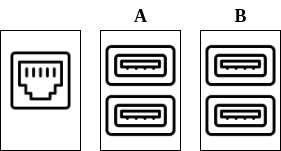
\includegraphics[scale=0.85]{F_Figures/usb_ports.png}
      \caption{USB blocks on Raspberry Pi.}
      \label{fig:usb_ports}
    \end{figure}

\end{itemize}

These steps provides all the necessary connections to complete the hardware assembly, except power supply. Once the power is connectred over micro-USB to the Raspberry, the system will start up.
Figure 3.4 shows the fully-connected system schema.
\\
\begin{figure}[htb]
  \centering
  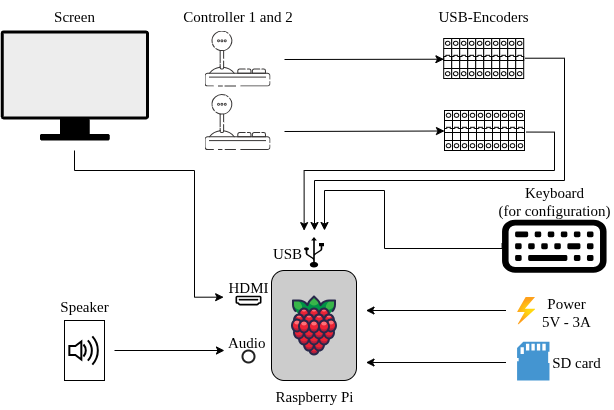
\includegraphics[scale=0.58]{F_Figures/system_schema.png}
  \caption{Fully-connected system schema.}
  \label{fig:system_schmema}
\end{figure}

\section{Running the System}
\label{sec:running_system}
Once the prepared SD card inserted into the Raspberry Pi, power the device on by pluging power cable. It is important to inserting SD card before powering on the device. After booting, the system will run on the RetroPie.
